\chapter{Full Film Magnetic Resonance}
\label{ch:FullFlimMagneticResonance}
In the following, the methods used to obtain the results presented in the results section as well as the optimization steps taken to ensure accurate measurements are outlined. 

\section{Measurement procedure}

To acquire an FMR spectrum, the field $\mathbf{H_\textrm{ext}}$ is swept while the microwave frequency and temperature $T$ are held constant. The resulting resonance curves are fitted to a Lorentzian function 
\begin{equation}
    L(H) =  A \left( \frac{-2(H - H_{\textrm{res}})\Delta H \cos(\phi) + ((\Delta H)^2 - (H - H_{\textrm{res}})^2) \sin(\phi)}{((H - H_{\textrm{res}})^2 + (\Delta H)^2)^2} \right) + C
\end{equation}
to extract key parameters like the resonance field $H_\textrm{res}$ and the linewidth $\Delta H$. $\phi$ represents the phase between the dispersive and absorptive part.
An exemplary set of FMR resonance curves is shown in figure \ref{Messung_FMR_Beispiel}. This procedure was then repeated for a range of 6 GHz to 24 GHz. After this was done for a single temperature, the temperature was changed and the procedure was repeated. For a single temperature, these two parameters were then plotted against the frequency of the RF signal. An example of such curves is shown in figure \ref{fig:Kittel_fits}.

\begin{figure}
\centering
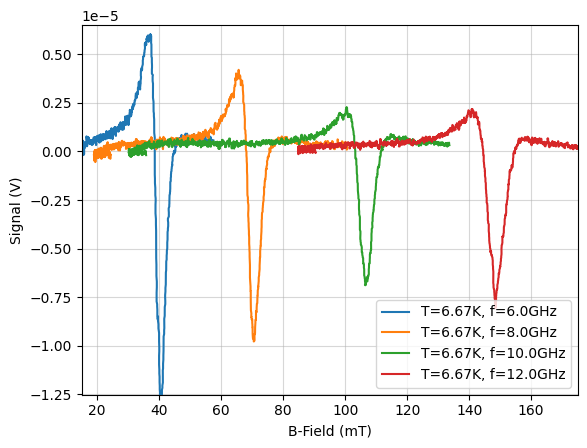
\includegraphics[width=0.6\textwidth]{chapters/Photos/Methods/FMRsample_MacOS.png}
\caption{Example of FMR resonance curves at a frequency of 6.67 K for various frequencies.}
\label{Messung_FMR_Beispiel}
\end{figure}

\begin{figure}[htbp] % [htbp] for flexible placement
    \centering % Center the entire figure
    \begin{subfigure}[c]{0.48\textwidth} 
        \subcaption{} % Place (a) above the image
        \centering
        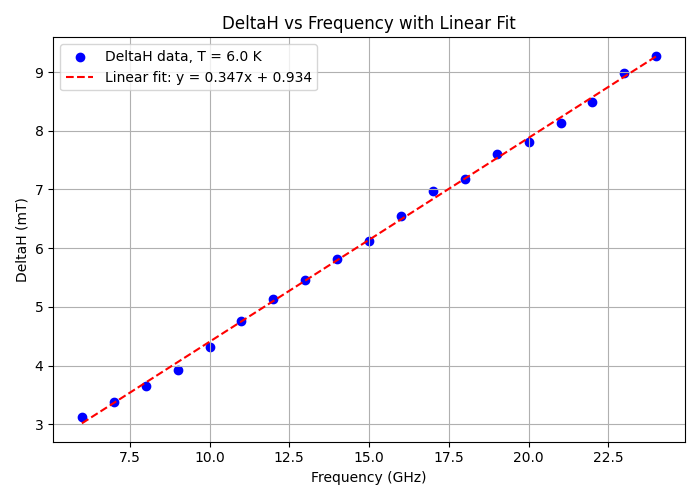
\includegraphics[width=\linewidth]{chapters/Photos/Methods/Kittellinear_macOS.png}
        \label{fig:Kittel_DltH}
    \end{subfigure}
    \hfill % Flexible horizontal space
    \begin{subfigure}[c]{0.48\textwidth} 
        \subcaption{} % Place (b) above the image
        \centering
        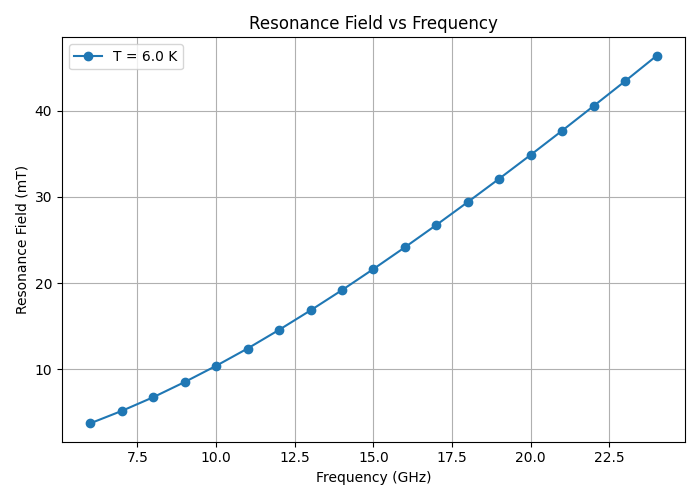
\includegraphics[width=\linewidth]{chapters/Photos/Methods/Kittelresonance_MacOS.png} 
        \label{fig:Kittel_Hres}
    \end{subfigure}
    \hfill % Flexible horizontal space
    \caption{Example of a resonance linewidth curve (a) and resonance field curve (b) at a temperature of 6 K for a Niobium layer thickness of $d_\textrm{Nb} = \SI{45}{nm}$. The resonance linewidth is fitted with a linear function (eq. \ref{linewidth equation}) and the resonance field is fitted with the Kittel formula (eq. \ref{Kittel equation}).}
    \label{fig:Kittel_fits} % Main label for the entire figure
\end{figure}

The resonance field and linewidth curves were fitted with the Kittel formula (\ref{Kittel equation}) and a linear function (\ref{linewidth equation}), respectively. The resonance field fit is used to extract $H_{\text{shift}}$, which corresponds to the shift of the resonance field from the expected value as explained in chapter \ref{ch:results} \cite{Jeon2019}, as well as $M_{\text{eff}}$, which is the effective magnetization. The linear fit of the linewidth curve is used to extract the Gilbert damping parameter $\alpha$ and the offset of the linewidth $\Delta H_0$.

Finally, these extracted parameters were plotted against the temperature to obtain the temperature dependence. These plots are shown in the results section below in figures \ref{fig:45nm_params} and \ref{fig:30nm_params}.

\section{Optimizing the RF signal power}
In order to obtain accurate measurements, the effect of the RF signal power on the FMR resonance curves was investigated with respect to the linewidth and the signal-to-noise ratio (SNR). The RF signal power was varied, and the resonance curves were compared to find the optimal power that maximizes SNR while still having no broadening effect of the resonance curve. For this purpose, the RF signal power was varied from 0 dBm to 10 dBm for a sample with $d_\textrm{Nb} = \SI{45}{nm}$ at a frequency of 10 GHz at a temperature of 7 K, which is around the critical temperature $T_\textrm{C}$. The results are shown in figure \ref{comparison_0dBmto10dBm_7K10Ghz}. From this comparison, it was concluded that the 10 dBm measurement provided the best SNR without significant broadening of the resonance curve. Due to the nature of the lock-in amplifier, the linewidth of the original resonance curve is actually shown in the peak-to-peak amplitude of the resonance curve.

\begin{figure}
\centering
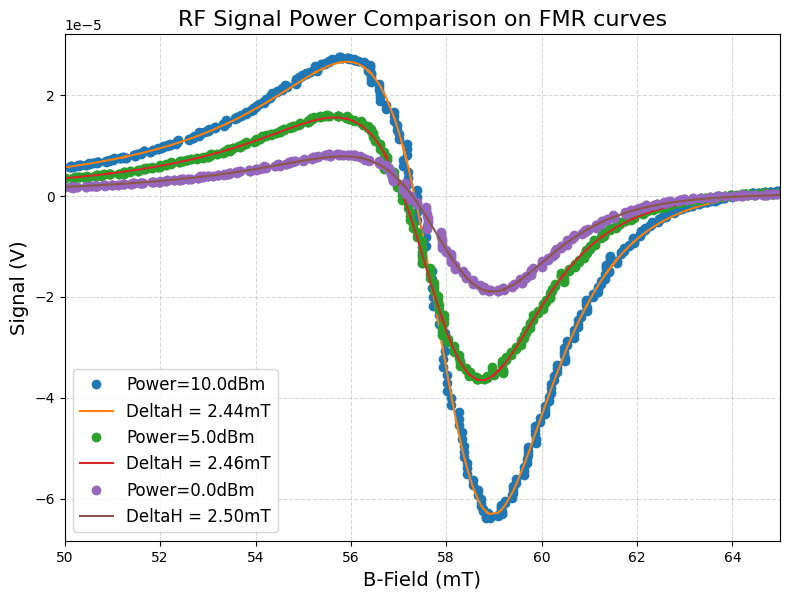
\includegraphics[width=0.8\textwidth]{chapters/Photos/Methods/RFSignalPower_MacOS.png}
\caption{Comparison of FMR resonance curves for $d_\textrm{Nb} = \SI{45}{nm}$ at a temperature of 7K and a frequency of 10GHz for different RF signal amplitudes.}
\label{comparison_0dBmto10dBm_7K10Ghz}
\end{figure}

\section{Optimizing the modulation field}
The modulation field, which is needed for the LIA to extract the FMR signal, was also optimized. Since the modulation field cannot be directly measured, due to the field sensor being located outside of the modulation coil, the effect of the modulation current which generates the modulation field was studied. A small modulation current would result in bad SNR, whereas a large modulation current would lead to increased linewidth broadening. The modulation current was varied from 0.01 A to 0.05 A for a sample with a $d_\textrm{Nb} = \SI{30}{nm}$ at a temperature of 5.6 K (which is near $T_\textrm{C}$) and a frequency of 8 GHz. The results are shown in figure \ref{comparison_0.01to0.05Ain30nm}. In the figure, it is visible that an increase in modulation current leads to an increase in linewidth broadening as well as a bigger amplitude and through that, a better SNR. From this comparison, it was concluded that an amplitude of 0.03 A is optimal, as it provides a good SNR while having minimal linewidth broadening. This test was done on both samples, though the conclusion remained the same.
\begin{figure}
\centering
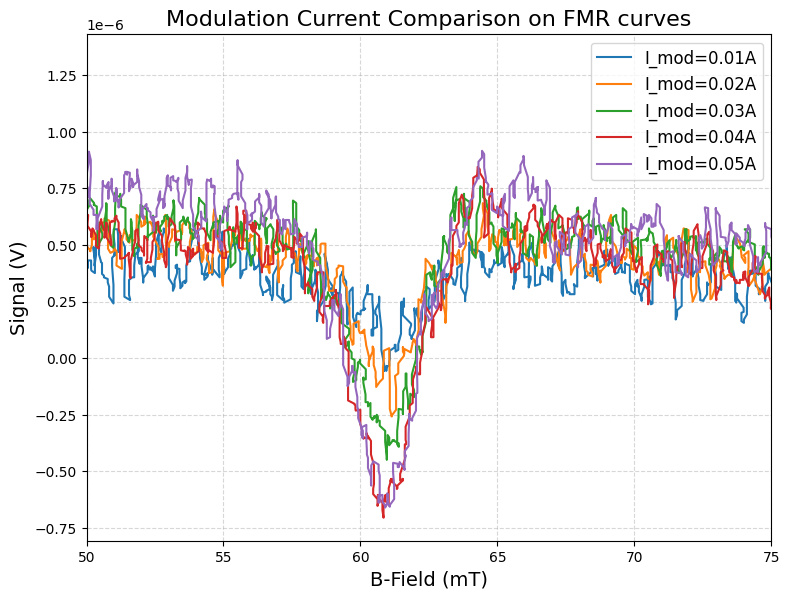
\includegraphics[width=0.8\textwidth]{chapters/Photos/Methods/Modcurrent_macOS.png}
\caption{Comparison of FMR resonance curves for a Niobium layer thickness of $d_\textrm{Nb} = \SI{30}{nm}$ at a temperature of 5.6K and a frequency of 8GHz for different RF signal amplitudes.}
\label{comparison_0.01to0.05Ain30nm}
\end{figure}


\section{Optimizing the Lock-in amplifier settings}
Finally, the settings of the lock-in amplifier (LIA) were optimized to achieve the best possible signal detection. For this, the time constant and the sensitivity of the LIA were adjusted. The time constant determines how quickly the LIA can respond to changes in the signal, while the sensitivity determines how small of a signal the LIA can detect. A larger time constant results in a slower response to changes in the signal, which can be beneficial for reducing noise but may also lead to a loss of signal fidelity. Conversely, a smaller time constant allows for a faster response but can increase the noise level in the measurement. The time constant and the sweep rate are interdependent, as a longer time constant requires a slower sweep rate to maintain measurement accuracy.
To optimize the measurement of a 45 nm thick sample ($d_\textrm{Nb} = \SI{45}{nm}$) at 7 K and 10 GHz, two settings were compared: A slow sweep at 0.05 A/min with a 1 s time constant, and a fast sweep at 0.1 A/min with a 0.3 s time constant. As shown in Figure \ref{fig:fast_and_slow}, the slower sweep and longer time constant offered no significant improvement to the SNR. Therefore, to prioritize measurement speed, the faster parameters (a sweep rate of 0.1 A/min and a time constant of 300 ms) was used for all subsequent experiments. Additionally, the LIA sensitivity was always set to the lowest possible range that did not cause signal clipping.

\begin{figure}
\centering
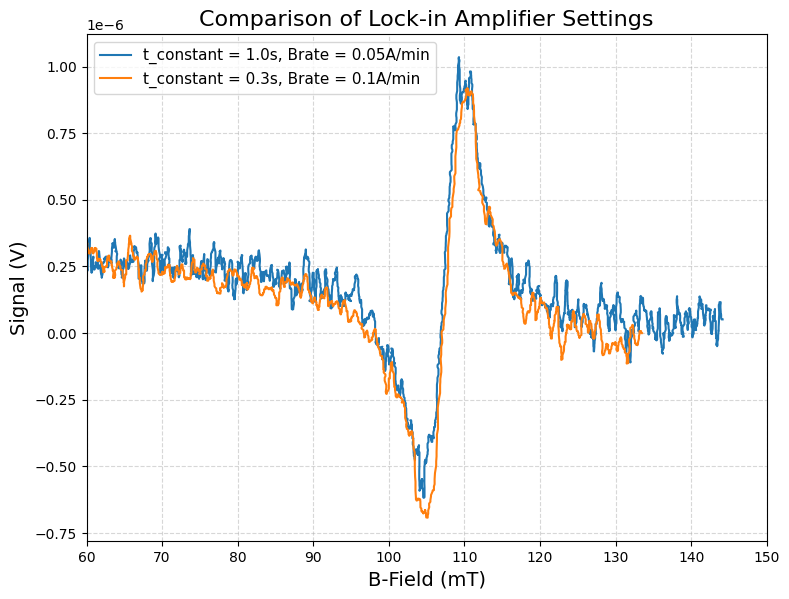
\includegraphics[width=0.8\textwidth]{chapters/Photos/Methods/TimeConstant_MacOS.png}
\caption{Comparison of FMR resonance curves for different sweep rates. The blue graph corresponds to the slow sweep rate (0.05 A/min) and higher time constant (1s), while the orange graph corresponds to the fast sweep rate (0.1 A/min) and lower time constant (300 ms). The measurements were done for a Niobium layer thickness of $d_\textrm{Nb} = \SI{45}{nm}$ at a temperature of 7K and a frequency of 10 GHz.}
\label{fig:fast_and_slow}
\end{figure}

